% Use only LaTeX2e, calling the article.cls class and 12-point type.

\documentclass[12pt]{article}

% Users of the {thebibliography} environment or BibTeX should use the
% scicite.sty package, downloadable from *Science* at
% www.sciencemag.org/about/authors/prep/TeX_help/ .
% This package should properly format in-text
% reference calls and reference-list numbers.

%\usepackage{scicite}

% Use times if you have the font installed; otherwise, comment out the
% following line.

\usepackage{times}
\usepackage{graphicx}
\usepackage{lettrine}
% The preamble here sets up a lot of new/revised commands and
% environments.  It's annoying, but please do *not* try to strip these
% out into a separate .sty file (which could lead to the loss of some
% information when we convert the file to other formats).  Instead, keep
% them in the preamble of your main LaTeX source file.


% The following parameters seem to provide a reasonable page setup.

\topmargin 0.0cm
\oddsidemargin 0.2cm
\textwidth 16cm 
\textheight 21cm
\footskip 1.0cm


%The next command sets up an environment for the abstract to your paper.

\newenvironment{sciabstract}{%
\begin{quote} \bf}
{\end{quote}}


% If your reference list includes text notes as well as references,
% include the following line; otherwise, comment it out.

\renewcommand\refname{References and Notes}

% The following lines set up an environment for the last note in the
% reference list, which commonly includes acknowledgments of funding,
% help, etc.  It's intended for users of BibTeX or the {thebibliography}
% environment.  Users who are hand-coding their references at the end
% using a list environment such as {enumerate} can simply add another
% item at the end, and it will be numbered automatically.

\newcounter{lastnote}
\newenvironment{scilastnote}{%
\setcounter{lastnote}{\value{enumiv}}%
\addtocounter{lastnote}{+1}%
\begin{list}%
{\arabic{lastnote}.}
{\setlength{\leftmargin}{.22in}}
{\setlength{\labelsep}{.5em}}}
{\end{list}}


% Include your paper's title here

\title{ Apriori implementation using Matlab} 


% Place the author information here.  Please hand-code the contact
% information and notecalls; do *not* use \footnote commands.  Let the
% author contact information appear immediately below the author names
% as shown.  We would also prefer that you don't change the type-size
% settings shown here.

\author
{Luting Chen  50133507,
	Yuze Liu 50207903, 
	Vicky Zheng  50037709 \\
%\normalsize{$^{1}$Department of Chemistry, University of Wherever,}\\
%\normalsize{An Unknown Address, Wherever, ST 00000, USA}\\
%\normalsize{$^{2}$Another Unknown Address, Palookaville, ST 99999, USA}\\
\\
%\normalsize{$^\ast$To whom correspondence should be addressed; E-mail:  jsmith@wherever.edu.}
}

% Include the date command, but leave its argument blank.

\date{}
%%%%%%%%%%%%%%%%% END OF PREAMBLE %%%%%%%%%%%%%%%%
\begin{document} 

% Double-space the manuscript.

\baselineskip24pt

% Make the title.

\maketitle 
% Place your abstract within the special {sciabstract} environment.

%\begin{sciabstract}
 % This document presents a number of hints about how to set up your
  %{\it Science\/} paper in \LaTeX\ .  We provide a template file,
  %\texttt{scifile.tex}, that you can use to set up the \LaTeX\ source
  %for your article.  An example of the style is the special
  %\texttt{\{sciabstract\}} environment used to set up the abstract you
  %see here.
%\end{sciabstract}
% In setting up this template for *Science* papers, we've used both
% the \section* command and the \paragraph* command for topical
% divisions.  Which you use will of course depend on the type of paper
% you're writing.  Review Articles tend to have displayed headings, for
% which \section* is more appropriate; Research Articles, when they have
% formal topical divisions at all, tend to signal them with bold text
% that runs into the paragraph, for which \paragraph* is the right
% choice.  Either way, use the asterisk (*) modifier, as shown, to
% suppress numbering.

\section*{Introduction}
The apriori algorithm is used to determine association rules. In this homework, we implemented the apriori algorithm by using Matlab. The dataset we used the algorithm on is gene data. The applications of this are straight forward: with association rules we can see how genes relate to each other and what the relation between genes can tell us about the data. 

\section*{Data Preprocesing}
\noindent The data provided is a .txt file that contains a 100 by 102 matrix. There are 100 samples each corresponding to the genes of a patient with a disease. The diseases are: ALL, AML, Breast Cancer and Colon Cancer. In order to optimize our program, we converted each of these values into integers: 1,2,3,4 respectively. The data set also gives us a sequence of 100 genes labeled as either up or down. Each gene at index i is treated as 1 if it is up and 0 if it is down. We did this to optimize our program by having fewer string comparsions since integer comparisons are much faster. 

\section*{Implementation}
\noindent For this homework, we choose to use Matlab because our input data is a matrix. Matlab has helpful functions for matrix manipulation like determining whether a set of numbers is in a row of the matrix. It also has helpful functions such as the union of two sets which helped us do the pruning necessary for an efficient apriori algorithm. In our implementation, we enumerate through all possible tuples where a tuple can be comprised of genes or genes and diseases. We start at the shortest length of tuples, and work our way up. We based our implementation off the diagram provided in class which is shown in Fig. 1. 

\begin{figure}[h]
	\centering
	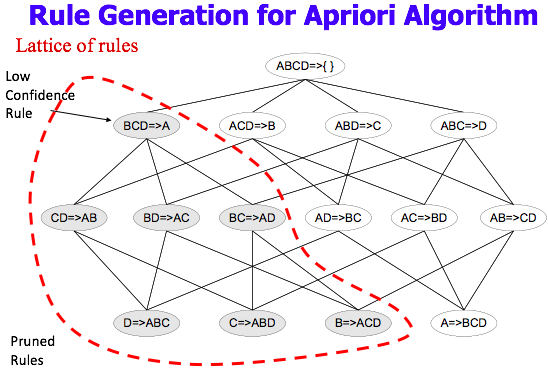
\includegraphics[width=\textwidth]{apriori}
	\caption{Apriori Pruning Search Space}
\end{figure}

Although our algorithm is O(n!) where n is the number of attributes, this pruning significantly reduces our runtime. This is because we expliot the fact that a superset of an infrequent set must also be infrequent. In Fig. 1, $$BCD=>A$$ was infrequent therefore all of it's supersets are also infrequent so we don't have to explore it. 

\section*{Results from Part 1}
\noindent With a support level of 30\%, we obtain the values: \\
196 of length 1 frequent item sets. \\
5340 of length 2 frequent item sets. \\
5287 of length 3 frequent item sets. \\
1518 of length 4 frequent item sets.\\
438 of length 5 frequent item sets.\\
88 of length 6 frequent item sets.\\
11 of length 7 frequent item sets.\\
1 of length 8 frequent item sets.\\

\noindent With a support level of 40\%, we obtain the values: \\
167 of length 1 frequent item sets. \\
753 of length 2 frequent item sets. \\
149 of length 3 frequent item sets. \\
7 of length 4 frequent item sets.\\
1 of length 5 frequent item sets.\\

\noindent With a support level of 50\%, we obtain the values: \\
109 of length 1 frequent item sets. \\
63 of length 2 frequent item sets. \\
2 of length 3 frequent item sets. \\

\noindent With a support level of 60\%, we obtain the values: \\
31 of length 1 frequent item sets. \\
2 of length 2 frequent item sets. \\

\noindent With a support level of 70\%, we obtain the values: \\
7 of length 1 frequent item sets. \\

\section*{Results from Part 2}
\noindent The results from Part 2 were obtained by combining our results from Part 1 and combining it with the counting method described in piazza post 113. Confidence is calculated from the equation: \\
$$c = \frac{\sigma(HEAD)}{\sigma(BODY)}$$
\begin{enumerate} 
	\item RULE HAS ANY OF G6\_UP \\
	Result: \\
	\item RULE HAS 1 OF G1\_UP \\
	Result: \\
	\item RULE HAS 1 OF (G1\_UP, G10\_DOWN) \\
	Result: \\
	\item BODY HAS ANY OF G6\_UP \\
	Result: \\
	\item BODY HAS NONE OF G72\_UP\\
	Result: \\
	\item BODY HAS 1 OF (G1\_UP, G10\_DOWN)\\
	Result: \\
	\item HEAD HAS ANY OF G6\_UP\\
	Result: \\
	\item HEAD HAS NONE OF (G1\_UP, G6\_UP)\\
	Result: \\
	\item HEAD HAS 1 OF (G6\_UP, G8\_UP)\\
	Result: \\
	\item RULE HAS 1 OF (G1\_UP, G6\_UP, G72\_UP)\\
	Result: \\
	\item RULE HAS ANY OF (G1\_UP, G6\_UP, G72\_UP)\\
	Result: \\

	\item SIZE OF RULE >= 3 \\
	Result: \\
	\item SIZE OF BODY >= 2 \\
	Result: \\
	\item SIZE OF HEAD >= 2 \\
	Result: \\

	\item  BODY HAS ANY OF G1\_UP AND HEAD HAS 1 OF G59\_UP \\
	Result: \\
	\item  BODY HAS ANY OF G1\_UP OR HEAD HAS 1 OF G6\_UP \\
	Result: \\
	\item  BODY HAS 1 OF G1\_UP OR HEAD HAS 2 OF G6\_UP \\
	Result: \\
	\item  HEAD HAS 1 OF G1\_UP AND BODY HAS 0 OF DISEASE \\
	Result: \\
	\item  HEAD HAS 1 OF DISEASE OR RULE HAS 1 OF (G72\_UP, G96\_DOWN) \\
	Result: \\
	\item  BODY HAS 1 of (G59\_UP, G96\_DOWN) AND SIZE OF RULE >=3 \\
	Result: \\
\end{enumerate}
\section*{Conclusion}

In this homework, we implemented the apriori algorithm to find association rules. With our implementation, we calculated the number of frequent sets for various lengths for support levels ranging from 0.3-0.7. With the frequent item sets, we are able to calculate the results from the queries given to us on piazza. We are able to do this because we have already calculated the frequent item sets for Support = .5 and we can easily calculate the confidence with the equation given to us to see if it means the threshold of .6. 

% Your references go at the end of the main text, and before the
% figures.  For this document we've used BibTeX, the .bib file
% scibib.bib, and the .bst file Science.bst.  The package scicite.sty
% was included to format the reference numbers according to *Science*
% style.

\bibliography{scibib}

\bibliographystyle{Science}

\begin{thebibliography}{9}
	\bibitem{latexcompanion} 
	Jing Gao
	\textit{Association1 Slides}. 

\end{thebibliography}


\end{document}




















